\documentclass{article}
\usepackage[frenchb]{babel}
\usepackage[utf8]{inputenc}
\usepackage[T1]{fontenc}
\usepackage{graphicx}
\usepackage{fancyhdr}
\usepackage{float}
\usepackage{hyperref}

\pagestyle{fancy}
\title{Projet d'interface Homme-Machine : \bsc{Quelle Est Cette Note}}
\author{Thibault \bsc{Béziers La Fosse}, Dennis \bsc{Bordet}}




\begin{document}

\renewcommand{\contentsname}{Sommaire} 


\maketitle
\date


\begin{figure}[h]

\begin{center}
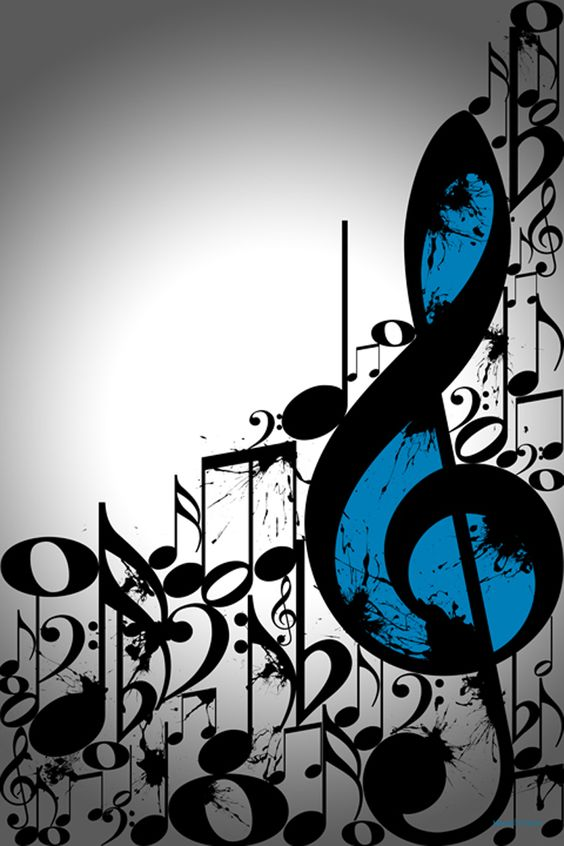
\includegraphics[width = 250px]{./images/deb2.jpg}
\end{center}

\end{figure}






\newpage

\tableofcontents

\newpage

\section{Introduction}

\vspace{1cm}

\subsection{Motivation et but du projet}

\vspace{1cm}
Pourquoi apprendre le solfège ? Afin d'éviter des catastrophes auditives comme le \href{https://www.youtube.com/watch?feature=player_detailpage&v=KolfEhV-KiA#t=18}{thème de titanic par Marc Mulholland}.

L'idée est de réaliser un petit logiciel pour initier les débutants au solfège. Il fallait donc au départ restreindre le programme,
le domaine de la musique étant assez vaste. Il a donc été décidé collégialement que le programme aurait un niveau assez faible et 
simple, niveau 6e en musique.


\subsection{Interface générale}

\vspace{1cm}

Il faut donc que l'utilisateur sache lire une partition simple en clef de sol, la partition ne contient que deux gammes.

L'outil choisi pour entrer les notes est un clavier de piano. Le piano étant un instrument universel en musique.

Il a également été décidé de représenter les \#
{ }et les b-mol, ceux-ci étant présent dans de très nombreuses partitions, il est donc
important pour un débutant d'en prendre connaissance.


\subsection{Plan}
\begin{itemize}
\item Explications des choix de l'interface
\item Paper prototype et compte rendu des essais
\item Test du logiciel par des cobayes
\end{itemize}

\newpage
\section{Différents éléments de l'interface}

\subsection{Portée}
\subsubsection{Variabilité de la portée}
Le but de notre application étant d'apprendre à lire une partition, il va de soi que notre logiciel devait contenir une portée de notes. 
Nous voulions pouvoir efficacement des portées de moins d'une dizaine de lignes, et des portées plus longues. Si bien que notre application adapte son affichage au nombre de notes. Arbitrairement, nous avons fixé le nombre de notes par ligne à 14. Nous estimons que c'est un juste milieu entre une portée trop pleine, et une portée trop vide.
\begin{center}
\begin{tabular}{cc}

	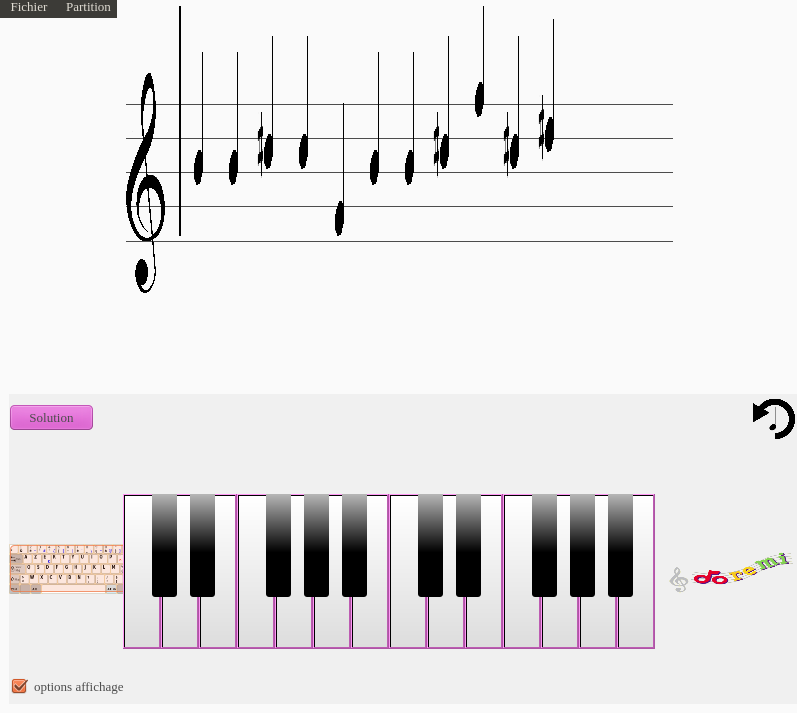
\includegraphics[width = 150px]{./images/1Line.png}

	&

	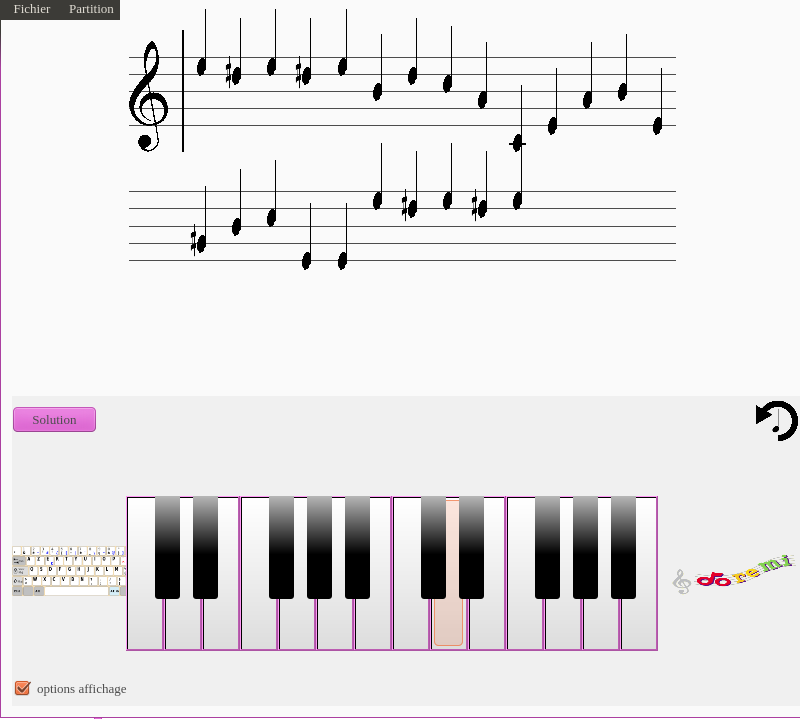
\includegraphics[width = 150px]{./images/2Line.png}

	\\
\end{tabular}
\end{center}

\subsubsection{Clef de sol \& Notes}
Le placement des notes et de la clef de sol dans la portée pouvait se faire de deux manières différentes avec \emph{Qt} : En dessinant les notes, ou en insérant des images. Nous avons tout d'abord choisi d'insérer la clef de Sol au début de la portée, car il aurait été impossible d'en dessiner une d'une manière propre. Ensuite nous avons commencé en dessinant les notes. Enfin nous avons vite changé d'avis, et inséré des images à la place, la variété des notes (Couleur, Dièse, normale, barrées ...) rendait le code illisible. L'insertion d'images nous a paru bien plus évidente, en plus d'être graphiquement plus agréable. 
\subsubsection{Curseur de suivi}
Afin de simplifier la lecture des notes par l'utilisateur, nous avons ajouté un curseur de lecture sur la portée. Il se présente sous la forme d'une barre verticale, de largeur 2px, et se positionne avant la prochaine note à jouer. A chaque note jouée, le curseur avance d'une note, ou bien recule d'une note si l'utilisateur annule sa dernière entrée. 
\begin{center}
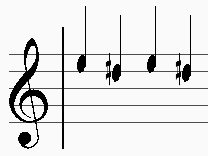
\includegraphics[width = 125px]{./images/scroller.png}
\end{center}
\subsubsection{Correction}
Lorsque l'utilisateur entre la dernière note de la portée, la correction débute automatiquement. Toutes les notes sont redessinées dans un vert léger, et volontairement non-agressif. Ensuite les entrées de l'utilisateur sont analysées. Chaque note est comparée à la partition. Lorsque la note est bien jouée, la note verte est donc simplement présente. Lorsque l'utilisateur s'est trompé, on place une note rouge correspondant à celle qu'il a joué, et une verte là où il aurait dû jouer. Ainsi il peut comprendre ses erreurs, et éventuellement recommencer en évitant de faire les mêmes erreurs. 
\begin{center}
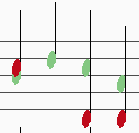
\includegraphics[width = 125px]{./images/correct.png}
\end{center}
\subsection{Menu}
Afin de naviguer dans notre application nous avons implémenté une barre d'outils. Cette barre propose 2 onglets, le premier, "Fichier", contient:

\begin{itemize}
\item Ouvrir un fichier, ou bien CTRL+O pour les utilisateurs de raccourcis, ouvre un fichier contenant une partition et l'affiche sur la portée. L'utilisateur peut ensuite la jouer.
\item Jouer en mode libre, qui permet de n'utiliser aucune partition, et de jouer librement du piano. Pour composer, par exemple.
\item Historique des scores, afin d'afficher sa progression, notamment au niveau des temps de réalisation, ainsi que des pourcentages de réussite.
\item Quitter, ou CTRL+Q, afin de fermer l'application. 
\end{itemize}
\begin{center}
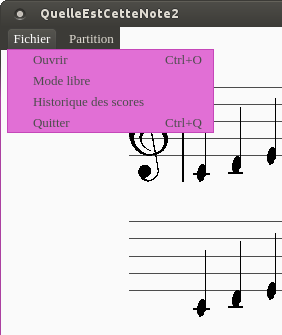
\includegraphics[width = 125px]{./images/toolBar.png}
\end{center}
Néanmoins suite à un problème d'implémentation nous avons fait un second onglet, "Partition", qui permet de choisir la partition dans un menu déroulant. Cependant, l'ouverture de partition étant constamment répétée, nous avons rapidement remarqué qu'un onglet de la barre d'outil destiné à cet effet était extrêmement plaisant. 

Finalement nous avons même ajouté un bouton \emph{+} en haut à gauche, accélérant d'autant plus l'accès au choix de partition. 

\subsection{Couleur de fond}
Nous avons choisit de mettre le fond en blanc, le blanc rendant la portée plus visible.
Le l'arrière plan du piano est quant à lui légèrement grisé pour faire une petite séparation entre la partition et le 
``groupe utilisateur'' (piano + boutons).
\subsection{Piano}
\subsubsection{Pourquoi le Piano ?}
Nous avons choisit de représenter uniquement un piano comme instrument, le métallophone étant très similaire, nous avons
jugé inutile d'en faire un. Pour d'autre instruments tel que le trombone, les notes auraient été plus difficiles à représenter,
moins parlantes. Le logiciel doit rester simple et pour débutants.
\subsubsection{Interactions}
Quand l'utilisateur appuie sur une touche du piano (avec la souris ou le clavier),
le programme lui confirme son action par une réponse visuelle et auditive.
En effet, la note est jouée et la touche du piano est enfoncée. De plus si l'utilisateur était en plein test sur une partition,
le curseur avance à chaque note tapée.
\subsubsection{Couleurs}
Les couleurs sont bien évidemment noires et blanches comme un piano normal. Nous avons décidé de donner un effet de lumière 
sur la partie haute du piano, les touches noires étant donc blanchies aux sommets. Ceci est un choix purement esthétique et 
apporte un effet plus réaliste au piano.
\subsubsection{Bulle d'information}
Pour chaque touche du piano, si l'utilisateur peut afficher la bulle d'information (tooltip), qui lui indiquera le nom de la 
note et son raccourci clavier. Eh oui, il y a des raccourcis clavier !
\subsection{Raccourcis clavier}
Le but du logiciel est d'apprendre les bases du solfège, mais de les apprendre le plus professionnellement possible.
Il ne s’agit donc pas de savoir lire des partitions simple mais de les lire rapidement !
Et pour savoir si l'utilisateur lit une partitions rapidement, il faut qu'il ait pu la jouer rapidement.
Jouer une partition à la souris étant particulièrement sportif et imprécis lorsque l'on joue rapidement, il est nécessaire
de pouvoir la jouer avec le clavier, comme un musicien aurait fait avec un vrai piano.
\subsection{Affichage des raccourcis}
Si chaque touche du piano correspond à une touche du clavier, il serait judicieux d'indiquer à l'utilisateur quelles sont les touches
qui sont associées. Et ceci sans avoir à afficher les bulles d'informations les unes après les autres. Nous avons donc décidé d'implémenter
un moyen d'afficher sur chacune des notes, son raccourci clavier. Cette fonction est lancé par un bouton situé à proximité du piano, ce qui
est évident puisque la fonction agit sur le piano (principe de chépakoi).
Ce bouton est représenté par un clavier, ce qui est assez parlant pour un utilisateur qui aurait envie d'utiliser son clavier 
pour jouer du piano.
Bien sûr, au cas où, une bulle d'information indique ce que fait ce bouton si un utilisateur moins futé se posait la question.
\subsection{Affichage du nom des notes}
De façon similaire, nous avons décidé d'implémenter une fonction indiquant la note de chaque touche. Le bouton qui la lance est lui 
aussi proche du piano. Par soucis de symétrie (et donc de confort visuel des utilisateurs), il est situé de l'autre coté de son semblable.
\'A quoi doit ressembler ce bouton: un petit dessin de clé de sol, avec les notes ``do re mi'' écrites est assez communiquant puisque
l'utilisateur peut voir le nom des trois premières notes sur ce bouton. Bien sur si ce n'est pas assez évident, le bulle d'information
est là.
Une question se pose alors : est-il possible d'afficher les raccourcis et les notes en même temps.
Oui, pourquoi pas après tout, si l'utilisateur en a envie, il ne faut pas l'en empêcher. Et ceci est tout à fait justifié si 
l'utilisateur débute avec le logiciel et le piano.
Cependant, nous n'avons pas pu l'implémenter sur notre programme car nous n'avons pas réussi à tout faire tenir sur la largeur de la touche
tout en étant lisible, ni à écrire sur plusieurs lignes dans la touche. Le temps qui nous était imparti étant assez court.
\subsection{Masquer les options}
\subsubsection{Pollution visuelle}
Certains utilisateurs, sûrement une majorité, une fois qu'ils seront familiers avec les notes et les raccourcis, ne voudront plus 
être embêtés par ces deux boutons qui ne leurs sont plus d'aucune utilité, nous avons donc décidé de pouvoir les cacher en décochant
une option.
\subsubsection{Optimisation de l'espace}
Ces deux boutons disparus, il reste de la place innocupée de chaque coté du piano, il est donc judicieux d'augmenter la taille 
du piano en conséquence, ce qui donne un meilleur confort visuel.

\subsubsection{Nom}
Cette fonction permettant d'améliorer l'espace de saisie des notes doit avoir un nom, pour indiquer à l'utilisateur ce qu'il va se 
passer. Le terme ``options d'affichage'' est plutôt parlant et à proximité du piano, il est probable que les options concernent le 
piano.
Le terme ``options'' lui est plus court mais il est moins précis. Quelles sont ces options ? Des touches supplémentaires ?
\subsection{Note de fin de session}
Le logiciel ayant un but éducatif, il faut donc évaluer l'utilisateur afin de determiner son niveau de connaissance.
Il y a deux critères pour l'évaluer:
\begin{itemize}
 \item Le nombre de bonnes réponses (en pourcentage)
 \item La vitesse à laquelle il a pu lire la partition
\end{itemize}
\'A la fin de chaque test (=partition), le récapitulatif de ces deux points est affiché accompgné d'une appréciation.
En plus, le personnage accompagnateur émet une petite remarque ayant pour but d'aider l'utilisateur à s'améliorer.
Par exemple, si l'utilisateur met plus de temps à trouver les notes en \# ou ``b-mol'', le personnage lui conseillera de les réviser.
Pour implémenter ceci, nous nous servons de différents fichiers de log.
\subsection{Progression}
En plus de la note de fin de session, les utilisateurs peuvent être intéressés par la progression de leurs notes et de leurs vitesse
de jeu. Il est donc intéressant de stocker un historique des scores, mais cette historique n'est pas consulté régulièrement, il ne 
faut donc pas que cette commande soit accessible directement sur l'écran principal et pollue l'espace.
\subsection{Choix de partitions}
Pour juger efficacement de l'évolution de l'utilisateur, il faut qu'il ait accès à un grand nombre de partitions, il ne faut donc 
pas les enregistrer ``en dur'' dans le programme, mais pouvoir les charger à partir d'un fichier ou autre. Cette commande étant utilisée
 souvent (enfin normalement), on peut la représenté par un petit ``+'' discret en haut a gauche de la partition.
 Bien sûr, cette commande est également présente dans le menu ``fichier->ouvrir'' pour les habitués aux logiciels de bureau.
 Il serait intéressant de tenir à jour un site qui repertorie de nombreuses partitions simples.
\subsection{Aide pour les débutants}
\subsubsection{Aide note apres note}
Et pour les tout débutants en solfège? Qui n'ont eu aucun cours sur le solfège ? Il faudrait pouvoir les aider lorsqu'ils sont 
vraiment bloqués dans l'ignorance. De ce fait, l'ajout d'un bouton qui donnerait indiquerait sur quelle touche appuyer.
Appeler cette touche ``solution'' est assez signifiant. ``Aide débutant'' étant plus vague et plus long.
\subsubsection{Partition modèle}
Il est aussi plus simple, pour quelqu'un qui n'a pas suivi un seul cours de solfège, d'avoir la possibilité d'avoir sous les yeux une
partitions avec toutes les notes des deux gammes du logiciel et leurs nom correspondant juste en dessous.
\subsection{Tutoriel au premier lancement}
Afin que l'utilisateur prenne parfaitement en main le logiciel, surtout les plus jeunes. Nous avons décidé (suite à un test sur cobaye numéro 1),
de lancer un petit tutoriel lors du premier démarrage. Ce tutoriel sérait dirigé par un personnage professeur accompagnant,
pas trop humain, un robot ou une note de musique vivante, c'est en tout cas ce qui ressort dans nos sondages.
Il expliquerait rapidement le but du programme, comment l'utiliser et comment avoir de l'aide en cas de besoin.
Ce serait aussi ce personnage qui donnerait les conseils et remarque à la fin de chaque test.





\section{Paper Prototype}
\subsection{Lien}
\href{https://www.youtube.com/watch?v=gwFMDVW2Swo}{Paper Prototype, 1er jet}.
\subsection{Essais et conséquences}
Suite à un essai du paper prototype par un des cobaye, ce dernier nous a fait remarquer que le bouton de correction ( présent dans la video )
est inutile puisque la correction est immédiatement lancée automatiquement lorsque le musicien en herbe joue sa dernière note. Et 
quel ``ahuri'' aurait l'idée de se faire évaluer sans avoir joué toutes ses notes!?
En effet, ce bouton semble bien inutile, nous avons donc décidé de le retirer.
\section{Test du logiciel par des cobayes}
\subsection{Cobaye numéro 1: Johnna, 6ans$1/2$, CP}

\begin{itemize}
\item \'A l'époque le logiciel n'avait pas de tutoriel. Le cobaye n'avait pas vraiment d'idée de ce qui allait se passer en cochant les 
options d'affichages. Mais une fois cliqué, il comprit.
\item Bouton ``do re mi'': le cobaye pensait que ce bouton allait lui jouer les notes do, ré et mi.
\item Le bouton permettant d'afficher les raccourcis clavier et celui pour donner la solution font parfaitement ce à quoi s'attendait
le cobaye.
\item Partition: le cobaye ne comprend pas vraiment la partition, l'intérêt de celle-ci
\end{itemize}

C'est ici que l'idée du tutoriel nous vient, il permettrait donc à se cobaye de savoir ce que font les boutons dont il ne savait pas
l'action et de le guider sur les partitions.

\subsection{Cobaye numéro 2:Charline}

Curseur trop petit.
Changement de taille du piano perturbant lors de l'affichage/masquage des options d'affichage.


\section{Conclusion}
Pour conclure ce rapport, ce fût vraiment un projet passionnant. Avant de commencer nous ne savions absolument rien faire avec Qt, hormis suivre les tutoriels, mais après avoir développé \emph{Quelle est cette note}, nous savons les bases pour écrire des applications complexes. C'est désormais un plus non négligeable à nos compétences. 

La conception de l'IHM de notre application nous a permis de réfléchir aux points vus en cours. Chaque partie fût l'objet d'une réflexion: Pourquoi ? Où ? Comment ? Afin d'obtenir un rendu final qui nous plaît. Même si notre application ne correspond pas tout à fait à notre \emph{Paper Prototype}, nous avons essayé de le suivre le plus fidèlement possible. 

Néanmoins, il reste toujours de nombreuses améliorations possibles à notre application: Amélioration des logs, une possible traduction des notes afin de s'ouvrir à l'internationale, avec un clavier compatible Qwerty. On pourrait aussi s'étendre sur plus de deux octaves, et même avec des clefs différentes. On pourrait aussi imaginer un outil de composition, écrivant sur la portée les notes entrées, au lieu de les lires. 

Enfin, on pourrait aussi trouver un nom mieux que \emph{Quelle est cette note}.
\end{document}

